\documentclass[12pt]{article}
\usepackage{amsmath,amsfonts,amssymb,amsthm} % Math packages
\usepackage[mathscr]{euscript}
\usepackage[utf8]{inputenc}
\usepackage[T1]{fontenc}
\usepackage{titling}
\usepackage[mathscr]{euscript}
\let\euscr\mathscr \let\mathscr\relax% just so we can load this and rsfs
\usepackage[scr]{rsfso}
\usepackage{pifont}
\usepackage{tikz}
\usepackage[dvipsnames]{xcolor}
\usepackage{geometry} % Adjust page margins
\usepackage{titlesec} % Adjust section and subsection formatting


\usetikzlibrary{automata,chains}
\geometry{a4paper, left=1in, right=1in, top=1in, bottom=1in}

\newcommand{\xlist}[1]{
    \begin{itemize}
        \renewcommand{\labelitemi}{$\centerdot$}
        #1
    \end{itemize}
    \newblock
}

\newcommand{\xsupposition}{
    \underline{Suppositions}:
    \\ \\
}

\newcommand{\xgoal}{
    \underline{Goal}:
    \\ \\
}

\newcommand{\xdeduction}{
    \underline{Deductions}:
    \\ \\
}

\newcommand{\xconclusion}{
    \underline{Conclusion}:
    \\ \\
}

\newcommand{\xproof}{
    \underline{Proof}:
    \\ \\
}

\newcommand{\xbasistep}{
    \underline{Basis Step}:
    \\ \\
}

\newcommand{\xinductivehypothesis}{
    \underline{Inductive Hypothesis}:
    \\ \\
}

\newcommand{\xinductivesteps}{
    \underline{Inductive Steps}:
    \\ \\
}

\title{
  \textbf{CS-225: Discrete Structures in CS} \\
  Assignment 9 Part 1
  }
\author{Noah Hinojos}
\date{\today}

\titleformat*{\subsection}{\normalsize\bfseries}

\begin{document}
\maketitle
\section*{Exercise Set 10.1}
\subsection*{2}
\begin{itemize}
  \item [a.] just a walk
  \item [b.] simple circuit
  \item [c.] closed walk
  \item [d.] circuit
  \item [e.] trail
  \item [f.] path
\end{itemize}
\subsection*{9 - b}
\begin{center}
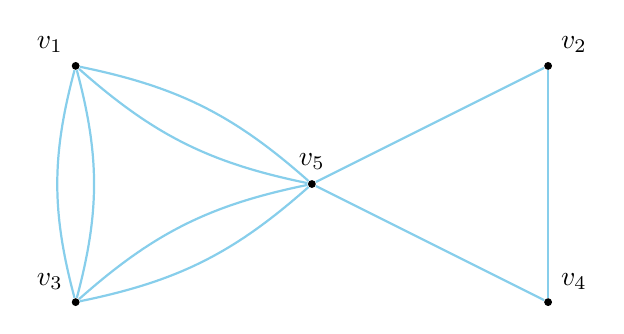
\begin{tikzpicture}[
  start chain=going right,
  roundnode/.style={draw,shape=circle,fill=blue,minimum size=1mm},
  ]
  \tikzset{%
    in place/.style={
      auto=false,
      fill=white,
      inner sep=2pt,
    },
  }
  %Nodes
  \node[circle,fill,inner sep=1pt,label={north west:$v_1$}](v1){};
  \node[circle,fill,inner sep=1pt,label={north east:$v_2$},xshift=5cm](v2)[right of=v1]{};
  \node[circle,fill,inner sep=1pt,label={north west:$v_3$},yshift=-2cm](v3)[below of=v1]{};
  \node[circle,fill,inner sep=1pt,label={north east:$v_4$},yshift=-2cm](v4)[below of=v2]{};
  \node[circle,fill,inner sep=1pt,label={north:$v_5$},yshift=-0.5cm, xshift=-3cm](v5)[below of=v2]{};
  %Lines
  \draw[-, auto]
    % Straight Line
    (v1) edge[color=SkyBlue, thick, bend left=15](v3)
    (v1) edge[color=SkyBlue, thick, bend right=15](v3)
    (v1) edge[color=SkyBlue, thick, bend left=15](v5)
    (v1) edge[color=SkyBlue, thick, bend right=15](v5)
    (v2) edge[color=SkyBlue, thick](v5)
    (v2) edge[color=SkyBlue, thick](v4)
    (v3) edge[color=SkyBlue, thick, bend left=15](v5)
    (v3) edge[color=SkyBlue, thick, bend right=15](v5)
    (v4) edge[color=SkyBlue, thick](v5)
    ;
\end{tikzpicture}
\end{center}
\newblock
\\
Yes, there is an Euler Circuit. Follow the vertices: 
$$v_5 v_2 v_4 v_5 v_1 v_3 v_5 v_1 v_3 v_5$$
Also by Theorem 10.1.4, graph $G$ must have an Euler Circuit.
\subsection*{15}
Yes, there is an Euler Circuit. Follow the vertices:
$$s r z y x w y u z s t u v w u s$$
\subsection*{20}
No, there is no Euler Circuit. 
By Theorem 10.1.4, there cannot exist an Euler Circuit because there are multiple vertices of odd degrees such as $u, e, h$ and $w$.
\subsection*{21}
Yes, there is an Euler Circuit. Follow the vertices:
$$u v_0 v_7 v_6 v_3 u v_1 v_2 v_3 v_4 v_6 w v_4 v_5 w$$
\end{document}
